\documentclass[12pt,a4paper]{article}
\usepackage{amsmath,amssymb,graphicx,float}
\usepackage[margin=2cm]{geometry}
\usepackage{hyperref}
\usepackage[utf8]{inputenc}
\usepackage{enumitem}
\usepackage{multicol}
\usepackage{booktabs}

\title{\textbf{Physics 11 Formulas}\\ Fundamental Constants and Equations}
\date{}
\begin{document}
\maketitle

\section{Physics Formulas}

\subsection{CH1,2,3: Kinematics}
\begin{align*}
\begin{array}{l@{\hspace{1.5cm}}l@{\hspace{1.5cm}}l}
\vec{v}=\frac{\Delta \vec{d}}{\Delta t} & \vec{a}=\frac{\Delta \vec{v}}{\Delta t} & v_{\mathrm{f}}=v_{\mathrm{i}}+a t \\[1em]
d=\left(\frac{v_{\mathrm{i}}+v_{\mathrm{f}}}{2}\right) t & d=v_{\mathrm{i}} t+\frac{1}{2} a t^{2} & v_{\mathrm{f}}^{2}=v_{\mathrm{i}}^{2}+2 a d \\[1em] 
d=d_0+\bar{v} t & \bar{v}=\frac{v_0+v_f}{2}  & v=v_0+a t \\[1em] 
d=d_0+v_0 t+\frac{1}{2} a t^2 & a=\frac{2 d}{t^2} \text{ (if } d_0=v_0=0\text{)} & v^2=v_0^2+2 a\left(d-d_0\right) 
\end{array}
\end{align*}

\subsection{CH4,5,6: Dynamics, Projectile Motion, and Rotational Motion}

\subsubsection{Newton's Laws and Forces (CH4.1-4.4)}
\begin{align*}
\begin{array}{l@{\hspace{1.5cm}}l@{\hspace{1.5cm}}l}
\text{First Law:} & \mathbf{F}_{\text{net}}=0 \text{ or } \Sigma \mathbf{F}=0 & \text{(equilibrium)} \\[1em]
\text{Second Law:} & \vec{F}_{\text{net}}=m\vec{a} & \mathbf{W}=m\mathbf{g} \\[1em]
\text{Forces:} & F_{\mathrm{g}}=G \frac{m_{1} m_{2}}{r^{2}} & F_{\mathrm{f}}=\mu F_{\mathrm{N}} \\[1em]
F_{\mathrm{s}}=k \Delta x & \mathbf{N}=m\mathbf{g} \text{ (horizontal)} & \mathbf{T}=m\mathbf{g} \text{ (at rest)}
\end{array}
\end{align*}

\subsubsection{Projectile Motion (CH5.1-5.3)}
\begin{align*}
\begin{array}{l@{\hspace{1.5cm}}l}
h=\frac{\mathbf{v}_{0y}^2}{2\mathbf{g}} & R=\frac{\mathbf{v}_0^2 \sin 2\theta_0}{\mathbf{g}}
\end{array}
\end{align*}

\subsubsection{Rotational Motion (CH6.1-6.2)}
\begin{align*}
\begin{array}{l@{\hspace{1.5cm}}l@{\hspace{1.5cm}}l}
\text{Angle \& Angular Velocity:} & \Delta \theta=\frac{\Delta s}{r} & \omega=\frac{\Delta \theta}{\Delta t} \\[1em]
\text{Tangential Speed:} & v=r\omega & \\[1em]
\text{Centripetal Motion:} & \mathbf{a}_{\mathrm{c}}=\frac{v^2}{r}=r\omega^2 & \mathbf{F}_{\mathrm{c}}=m\frac{v^2}{r}=mr\omega^2
\end{array}
\end{align*}

\subsection{CH8: Momentum}
\begin{align*}
\begin{array}{l@{\hspace{2cm}}l@{\hspace{2cm}}l}
\text{Linear momentum} & \mathbf{p}=m \mathbf{v} & \\[1em]
\text{Impulse-momentum theorem} & \Delta \mathbf{p}=\mathbf{F}_{\text{net}} \Delta t & \\[1em]
\text{Conservation of momentum} & \mathbf{p}_{\text{tot}}= \text{constant}, \text{ or } \mathbf{p}_{\text{tot}}=\mathbf{p}_{\text{tot}}^{\prime} & \\[1em]
\text{Elastic collision (1D)} & m_1 \mathbf{v}_1+m_2 \mathbf{v}_2=m_1 \mathbf{v}_1^{\prime}+m_2 \mathbf{v}_2^{\prime} & \\[1em]
\text{2D collision (x-axis)} & m_1\mathbf{v}_1=m_1\mathbf{v}_1^{\prime}\cos\theta_1+m_2\mathbf{v}_2^{\prime}\cos\theta_2 & \\[1em]
\text{Angular momentum} & \mathbf{L}=I \omega &
\end{array}
\end{align*}
\subsection{CH9: Work, Energy, and Power}

\subsubsection{Work, Power, and Work-Energy Theorem}
\begin{align*}
\begin{array}{l@{\hspace{1.5cm}}l@{\hspace{1.5cm}}l}
\text{Kinetic Energy:} & KE=\frac{1}{2}m\mathbf{v}^2 & \\[1em]
\text{Work:} & W=\mathbf{f}d & \\[1em]
\text{Power:} & P=\frac{W}{t} & \\[1em]
\text{Work Equivalencies:} & W= PE_e=\Delta KE=\mathbf{f}m\mathbf{g}=\frac{1}{2}m\mathbf{v}_2^2-\frac{1}{2}m\mathbf{v}_1^2 &
\end{array}
\end{align*}

\subsubsection{Conservation of Energy}
\begin{align*}
KE_1 + PE_1 = KE_2 + PE_2
\end{align*}

\subsubsection{Simple Machines}
\begin{align*}
\begin{array}{l@{\hspace{1cm}}l@{\hspace{1cm}}l}
\text{General IMA:} & \text{Lever IMA:} & \text{Wheel and Axle IMA:} \\
IMA=\frac{\mathbf{F}_r}{\mathbf{F}_e}=\frac{d_e}{d_r} & IMA=\frac{L_e}{L_r} & IMA=\frac{R}{r} \\[1em]
\text{Inclined Plane IMA:} & \text{Wedge IMA:} & \text{Pulley IMA:} \\
IMA=\frac{L}{h} & IMA=\frac{L}{t} & IMA=N \\[1em]
\text{Screw IMA:} & \text{Input Work:} & \text{Output Work:} \\
IMA=\frac{2\pi L}{P} & W_i=\mathbf{F}_id_i & W_o=\mathbf{F}_od_o \\[1em]
\multicolumn{3}{l}{\text{Efficiency: } \text{\% efficiency}=\frac{W_o}{W_i} \times 100}
\end{array}
\end{align*}

\subsection{CH11: Thermal Physics}

\subsubsection{Temperature and Thermal Energy}
\begin{align*}
\begin{array}{l@{\hspace{1cm}}l@{\hspace{1cm}}l}
\text{C} \rightarrow \text{F:} & \text{C} \rightarrow \text{K:} & \text{F} \rightarrow \text{K:} \\
T^{\circ}_\mathrm{F} = \frac{9}{5}T^{\circ}_\mathrm{C} + 32 & T_\mathrm{K} = T^{\circ}_\mathrm{C} + 273.15 & T_\mathrm{K} = \frac{5}{9}(T^{\circ}_\mathrm{F} - 32) + 273.15 \\[1em]
\text{F} \rightarrow \text{C:} & \text{K} \rightarrow \text{C:} & \text{K} \rightarrow \text{F:} \\
T^{\circ}_\mathrm{C} = \frac{5}{9}(T^{\circ}_\mathrm{F} - 32) & T^{\circ}_\mathrm{C} = T_\mathrm{K} - 273.15 & T^{\circ}_\mathrm{F} = \frac{9}{5}(T_\mathrm{K} - 273.15) + 32
\end{array}
\end{align*}

\subsubsection{Heat, Specific Heat, and Heat Transfer}
\begin{align*}
\begin{array}{l@{\hspace{1.5cm}}l}
\text{Heat Transfer:} & Q = mc\Delta T \\[1em]
\text{Density:} & \rho = \frac{m}{V}
\end{array}
\end{align*}

\subsubsection{Phase Change and Latent Heat}
\begin{align*}
\begin{array}{l@{\hspace{1.5cm}}l}
\text{Heat Transfer (Melting/Freezing):} & Q = mL_f \\[1em]
\text{Heat Transfer (Vaporization/Condensation):} & Q = mL_v
\end{array}
\end{align*}

\subsection{CH12: Laws of Thermodynamics}
\begin{multicols}{2}
\begin{align*}
\text{First Law: } & \Delta U = Q - W \\
\text{Pressure: } & P = \frac{F}{A} \\
\text{P-V Work: } & W = P\Delta V \\
\text{Ideal Gas Law: } & PV = NkT 
\end{align*}

\columnbreak

\begin{align*}
\text{Entropy Change: } & \Delta S = \frac{Q}{T} \\
\text{Heat Engine Efficiency: } & Eff = \frac{W}{Q_h} \\
\text{Cyclical Work: } & W = Q_h - Q_c
\end{align*}
\end{multicols}

\subsection{CH5.5: Simple Harmonic Motion}
\begin{align*}
\begin{array}{l@{\hspace{1.5cm}}l}
\vec{F} = -k\vec{x} \text{ (Hooke's Law)} & T = 2\pi\sqrt{\frac{m}{k}}, \quad f = \frac{1}{2\pi}\sqrt{\frac{k}{m}} \\[1em] 
T = 2\pi\sqrt{\frac{L}{g}} \text{ (Simple Pendulum)} & \\
\end{array}
\end{align*}

\subsection{CH13-14: Waves and Sound}
\begin{align*}
\begin{array}{l@{\hspace{1.5cm}}l}
v = f\lambda, \quad T = \frac{1}{f}, \quad f = \frac{1}{T} & I = \frac{P}{A}, \quad I = \frac{(\Delta p)^2}{2\rho v_w}, \quad \beta \text{ (dB)} = 10\log_{10}\left(\frac{I}{I_0}\right) \\[1em]
f_{obs} = f_s\left(\frac{v_w}{v_w \pm v_s}\right) \text{ (moving source)} & f_{obs} = f_s\left(\frac{v_w \pm v_{obs}}{v_w}\right) \text{ (moving observer)} \\[1em]
f_B = |f_1 - f_2| \text{ (beat frequency)} & f_n = n\frac{v}{4L}, \, n = 1,3,5... \text{ (closed pipe)} \\[1em]
f_n = n\frac{v}{2L}, \, n = 1,2,3... \text{ (open pipe)} & \\
\end{array}
\end{align*}

\subsection{CH18: Electric Fields and Potential}
\begin{align*}
\begin{array}{l@{\hspace{1.5cm}}l}
\text{Coulomb's Law: } F = \frac{k q_1 q_2}{r^2} & \vec{E} = \frac{\vec{F}}{q_{\text{test}}}, \quad E = \frac{k|Q|}{r^2} \\[1em]
\Delta U_E = -qE(x_f - x_i) & U_E = \frac{kQq}{r} \\[1em]
\Delta V = -E(x_f - x_i) & V = \frac{kQ}{r} \\[1em]
C = \frac{Q}{V}, \quad U_E = \frac{1}{2}CV^2 & C = \kappa\varepsilon_0\frac{A}{d}
\end{array}
\end{align*}

\subsection{CH19: Current, Resistance, and Circuits}
\begin{align*}
\begin{array}{l@{\hspace{1.5cm}}l}
I = \frac{\Delta Q}{\Delta t}, \quad \text{1 A} = \text{1 C/s} & \text{Ohm's Law: } V = IR \\[1em]
\text{Series: } R_{\text{equiv}} = R_1 + R_2 + \cdots + R_N & \text{Parallel: } R_{\text{equiv}} = \frac{1}{1/R_1 + 1/R_2 + \cdots + 1/R_N} \\[1em]
P = IV & P = I^2R = \frac{V^2}{R}
\end{array}
\end{align*}



\iffalse

\subsection{CH8,9: Momentum, Work, Energy, and Power}
\begin{align*}
\begin{array}{l@{\hspace{2cm}}l@{\hspace{2cm}}l}
E_{\mathrm{k}}=\frac{1}{2} m v^{2} & E_{\mathrm{p}}=m g h & W=\vec{F} \cdot \vec{d} \\[1em]
W=\Delta E & P=\frac{W}{\Delta t}=\frac{\Delta E}{\Delta t} & \text{efficiency}=\frac{W_{\text {out }}}{W_{\text {in }}}=\frac{P_{\text {out }}}{P_{\text {in }}}
\end{array}
\end{align*}
\subsection{CH9: Simple Machines and Mechanical Advantage}
\begin{align*}
\begin{array}{l@{\hspace{2cm}}l@{\hspace{2cm}}l}
\text{(No specific formulas provided)} & &
\end{array}
\end{align*}
\subsection{CH11,12: Thermal Physics}
\begin{align*}
\begin{array}{l@{\hspace{2cm}}l@{\hspace{2cm}}l}
\text{(No specific formulas provided)} & &
\end{array}
\end{align*}
\subsection{CH13,14: Waves and Sound}
\begin{align*}
\begin{array}{l@{\hspace{2cm}}l@{\hspace{2cm}}l}
T=\frac{1}{f} & &
\end{array}
\end{align*}
\subsection{CH18,19: Electricity and Circuits}
\begin{align*}
\begin{array}{l@{\hspace{2cm}}l@{\hspace{2cm}}l}
I=\frac{Q}{\Delta t} & R=\frac{\rho \ell}{A} & V=I R \\[1em]
P=V I & R_{\mathrm{s}}=\sum_{i} R_{i} & \frac{1}{R_{\mathrm{p}}}=\sum_{i} \frac{1}{R_{i}} \\[1em]
V_{\text {terminal }}=\varepsilon \pm I r & &
\end{array}
\end{align*}

\fi

\newpage
\section{Mathematical Formulas}

\subsection{Right-angled Triangles}

\begin{figure}[H]
    \centering
    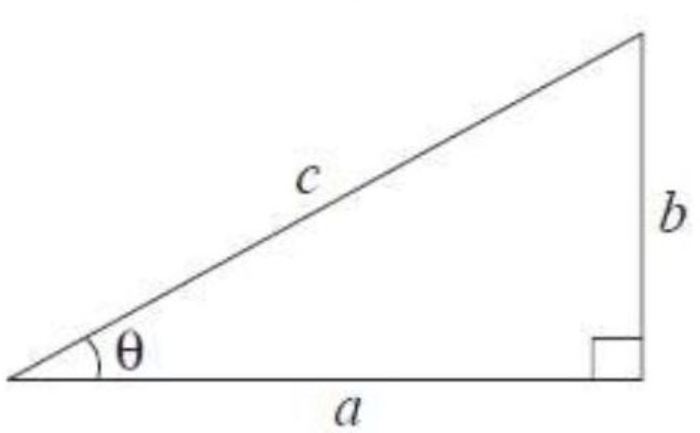
\includegraphics[width=0.4\linewidth]{11 Formula Sheet/rt.png}
    \caption{Right-angled triangle}
    \label{fig:Right-angled triangle}
\end{figure}

\begin{align*}
  \begin{array}{l@{\hspace{2cm}}l@{\hspace{2cm}}l}
    a^2 + b^2 = c^2 & \sin \theta = \frac{b}{c} & \cos \theta = \frac{a}{c} \\[1em]
    \tan \theta = \frac{b}{a} & \text{area} = \frac{1}{2}ab &
  \end{array}
\end{align*}

\subsection{All Triangles}
\begin{figure}[H]
    \centering
    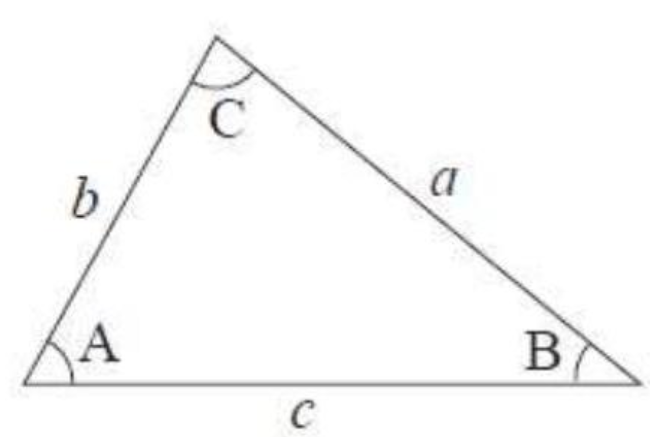
\includegraphics[width=0.4\linewidth]{11 Formula Sheet/nrt.png}
    \caption{Non-Right-angled triangle}
    \label{fig:Non-Right-angled triangle}
\end{figure}

\begin{align*}
  \begin{array}{l@{\hspace{2cm}}l@{\hspace{2cm}}l}
    \text{area} = \frac{1}{2} \text{base} \times \text{height} & \text{Sine Law:} \quad \frac{\sin A}{a} = \frac{\sin B}{b} = \frac{\sin C}{c} & \\[1em]
    \text{Cosine Law:} \quad c^2 = a^2 + b^2 - 2ab \cos C & &
  \end{array}
\end{align*}

\subsection{Circle and Sphere}
\begin{align*}
  \begin{array}{l@{\hspace{2cm}}l@{\hspace{2cm}}l}
    \text{Circle circumference:} \quad 2\pi r & \text{Circle area:} \quad \pi r^2 & \text{Sphere surface area:} \quad 4\pi r^2 \\[1em]
    \text{Sphere volume:} \quad \frac{4}{3}\pi r^3 & &
  \end{array}
\end{align*}

\subsection{Quadratic Equation}
For $ax^2 + bx + c = 0$: 
\[x = \frac{-b \pm \sqrt{b^2 - 4ac}}{2a}\]

\section{Metric Prefixes and Cardinal Directions}
\begin{figure}[H]
    \centering
    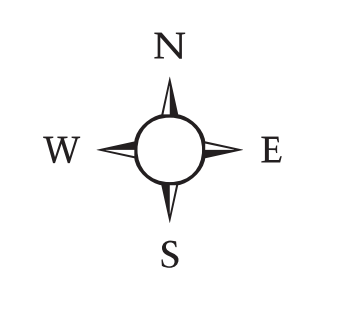
\includegraphics[width=0.4\linewidth]{11 Formula Sheet/nesw.png}
    \caption{Cardinal directions: North, South, East, and West}
    \label{fig:Cardinal directions}
\end{figure}

\begin{table}[H]
\centering
\begin{tabular}{@{}llcc@{}}
\toprule
Prefix & Symbol & Numerical & Exponential \\
\midrule
mega & M & 1000000 & $10^6$ \\
kilo & k & 1000 & $10^3$ \\
hecto & h & 100 & $10^2$ \\
deca & da & 10 & $10^1$ \\
 &  & 1 & $10^0$ \\
deci & d & 0.1 & $10^{-1}$ \\
centi & c & 0.01 & $10^{-2}$ \\
milli & m & 0.001 & $10^{-3}$ \\
micro & $\mu$ & 0.000001 & $10^{-6}$ \\
\bottomrule
\end{tabular}
\end{table}

\section{Fundamental Constants and Physical Data}

\begin{align*}
  \begin{array}{l@{\hspace{1cm}}r}
    \text{Gravitational constant:} & G=6.67 \times 10^{-11} \mathrm{Nm}^2/\mathrm{kg}^2 \\[1em]
    \text{Coulomb's Law constant:} & k=9.00 \times 10^9 \mathrm{Nm}^2/\mathrm{C}^2 \\[1em]
    \text{Elementary charge:} & e=1.60 \times 10^{-19} \mathrm{C} \\[1em]
    \text{Electron mass:} & m_e=9.11 \times 10^{-31} \mathrm{kg} \\[1em]
    \text{Proton mass:} & m_p=1.67 \times 10^{-27} \mathrm{kg} \\[1em]
    \text{Permeability of free space:} & \mu_0=4\pi \times 10^{-7} \mathrm{Tm}/\mathrm{A} \\[1em]
    \text{Speed of light:} & c=3.00 \times 10^8 \mathrm{m}/\mathrm{s}
  \end{array}
\end{align*}

\subsection{Earth}
\begin{align*}
  \begin{array}{l@{\hspace{1cm}}r@{\hspace{1cm}}l@{\hspace{1cm}}r}
    \text{Radius:} & 6.38 \times 10^6 \mathrm{m} & \text{Mass:} & 5.98 \times 10^{24} \mathrm{kg} \\[1em]
    \text{Surface gravity:} & g=9.81 \mathrm{m}/\mathrm{s}^2 & \text{Rotation period:} & 8.61 \times 10^4 \mathrm{s} \\[1em]
    \text{Orbit radius (Sun):} & 1.50 \times 10^{11} \mathrm{m} & \text{Orbit period (Sun):} & 3.16 \times 10^7 \mathrm{s}
  \end{array}
\end{align*}

\subsection{Moon}
\begin{align*}
  \begin{array}{l@{\hspace{1cm}}r@{\hspace{1cm}}l@{\hspace{1cm}}r}
    \text{Radius:} & 1.74 \times 10^6 \mathrm{m} & \text{Mass:} & 7.35 \times 10^{22} \mathrm{kg} \\[1em]
    \text{Rotation period:} & 2.36 \times 10^6 \mathrm{s} & \text{Orbit radius (Earth):} & 3.84 \times 10^8 \mathrm{m} \\[1em]
    \text{Orbit period (Earth):} & 2.36 \times 10^6 \mathrm{s} & \text{Surface gravity:} & 1.67 \, \mathrm{m/s^2}
\end{array}
\end{align*}

\subsection{Sun}
Mass: $1.98 \times 10^{30} \mathrm{kg}$

\end{document}